\documentclass[
  jou,
  floatsintext,
  longtable,
  nolmodern,
  notxfonts,
  notimes,
  colorlinks=true,linkcolor=blue,citecolor=blue,urlcolor=blue]{apa7}

\usepackage{amsmath}
\usepackage{amssymb}



\usepackage[bidi=default]{babel}
\babelprovide[main,import]{ngerman}


% get rid of language-specific shorthands (see #6817):
\let\LanguageShortHands\languageshorthands
\def\languageshorthands#1{}

\RequirePackage{longtable}
\RequirePackage{threeparttablex}

\makeatletter
\renewcommand{\paragraph}{\@startsection{paragraph}{4}{\parindent}%
	{0\baselineskip \@plus 0.2ex \@minus 0.2ex}%
	{-.5em}%
	{\normalfont\normalsize\bfseries\typesectitle}}

\renewcommand{\subparagraph}[1]{\@startsection{subparagraph}{5}{0.5em}%
	{0\baselineskip \@plus 0.2ex \@minus 0.2ex}%
	{-\z@\relax}%
	{\normalfont\normalsize\bfseries\itshape\hspace{\parindent}{#1}\textit{\addperi}}{\relax}}
\makeatother




\usepackage{longtable, booktabs, multirow, multicol, colortbl, hhline, caption, array, float, xpatch}
\setcounter{topnumber}{2}
\setcounter{bottomnumber}{2}
\setcounter{totalnumber}{4}
\renewcommand{\topfraction}{0.85}
\renewcommand{\bottomfraction}{0.85}
\renewcommand{\textfraction}{0.15}
\renewcommand{\floatpagefraction}{0.7}

\usepackage{tcolorbox}
\tcbuselibrary{listings,theorems, breakable, skins}
\usepackage{fontawesome5}

\definecolor{quarto-callout-color}{HTML}{909090}
\definecolor{quarto-callout-note-color}{HTML}{0758E5}
\definecolor{quarto-callout-important-color}{HTML}{CC1914}
\definecolor{quarto-callout-warning-color}{HTML}{EB9113}
\definecolor{quarto-callout-tip-color}{HTML}{00A047}
\definecolor{quarto-callout-caution-color}{HTML}{FC5300}
\definecolor{quarto-callout-color-frame}{HTML}{ACACAC}
\definecolor{quarto-callout-note-color-frame}{HTML}{4582EC}
\definecolor{quarto-callout-important-color-frame}{HTML}{D9534F}
\definecolor{quarto-callout-warning-color-frame}{HTML}{F0AD4E}
\definecolor{quarto-callout-tip-color-frame}{HTML}{02B875}
\definecolor{quarto-callout-caution-color-frame}{HTML}{FD7E14}

%\newlength\Oldarrayrulewidth
%\newlength\Oldtabcolsep


\usepackage{hyperref}




\providecommand{\tightlist}{%
  \setlength{\itemsep}{0pt}\setlength{\parskip}{0pt}}
\usepackage{longtable,booktabs,array}
\usepackage{calc} % for calculating minipage widths
% Correct order of tables after \paragraph or \subparagraph
\usepackage{etoolbox}
\makeatletter
\patchcmd\longtable{\par}{\if@noskipsec\mbox{}\fi\par}{}{}
\makeatother
% Allow footnotes in longtable head/foot
\IfFileExists{footnotehyper.sty}{\usepackage{footnotehyper}}{\usepackage{footnote}}
\makesavenoteenv{longtable}

\usepackage{graphicx}
\makeatletter
\newsavebox\pandoc@box
\newcommand*\pandocbounded[1]{% scales image to fit in text height/width
  \sbox\pandoc@box{#1}%
  \Gscale@div\@tempa{\textheight}{\dimexpr\ht\pandoc@box+\dp\pandoc@box\relax}%
  \Gscale@div\@tempb{\linewidth}{\wd\pandoc@box}%
  \ifdim\@tempb\p@<\@tempa\p@\let\@tempa\@tempb\fi% select the smaller of both
  \ifdim\@tempa\p@<\p@\scalebox{\@tempa}{\usebox\pandoc@box}%
  \else\usebox{\pandoc@box}%
  \fi%
}
% Set default figure placement to htbp
\def\fps@figure{htbp}
\makeatother


% definitions for citeproc citations
\NewDocumentCommand\citeproctext{}{}
\NewDocumentCommand\citeproc{mm}{%
  \begingroup\def\citeproctext{#2}\cite{#1}\endgroup}
\makeatletter
 % allow citations to break across lines
 \let\@cite@ofmt\@firstofone
 % avoid brackets around text for \cite:
 \def\@biblabel#1{}
 \def\@cite#1#2{{#1\if@tempswa , #2\fi}}
\makeatother
\newlength{\cslhangindent}
\setlength{\cslhangindent}{1.5em}
\newlength{\csllabelwidth}
\setlength{\csllabelwidth}{3em}
\newenvironment{CSLReferences}[2] % #1 hanging-indent, #2 entry-spacing
 {\begin{list}{}{%
  \setlength{\itemindent}{0pt}
  \setlength{\leftmargin}{0pt}
  \setlength{\parsep}{0pt}
  % turn on hanging indent if param 1 is 1
  \ifodd #1
   \setlength{\leftmargin}{\cslhangindent}
   \setlength{\itemindent}{-1\cslhangindent}
  \fi
  % set entry spacing
  \setlength{\itemsep}{#2\baselineskip}}}
 {\end{list}}
\usepackage{calc}
\newcommand{\CSLBlock}[1]{\hfill\break\parbox[t]{\linewidth}{\strut\ignorespaces#1\strut}}
\newcommand{\CSLLeftMargin}[1]{\parbox[t]{\csllabelwidth}{\strut#1\strut}}
\newcommand{\CSLRightInline}[1]{\parbox[t]{\linewidth - \csllabelwidth}{\strut#1\strut}}
\newcommand{\CSLIndent}[1]{\hspace{\cslhangindent}#1}





\usepackage{newtx}

\defaultfontfeatures{Scale=MatchLowercase}
\defaultfontfeatures[\rmfamily]{Ligatures=TeX,Scale=1}





\title{Evidenz.Besser.Kommunizieren.: Wie Bildungswissenschaften und
Fachdidaktiken ihre Wissenschaftskommunikation weiterentwickeln können.}


\shorttitle{Evidenz.Besser.Kommunizieren.}


\usepackage{etoolbox}









\authorsnames{Samuel Merk,Sarah Bez,Kirstin Schmidt}






\authorsaffiliations{
{Pädagogische Hochschule Karlsruhe},{}}




\leftheader{Merk, Bez and Schmidt}



\abstract{Lehrkräfte treffen tagtäglich unzählige Entscheidungen bzgl.
ihrer Unterrichtsgestaltung und -entwicklung. Dabei rekurrieren Sie
vornehmlich auf persönliche Erfahrung, Konzeptwissen oder Heuristiken.
Evidenz aus Bildungswissenschaften und Fachdidaktiken wird das Potential
zugeschrieben diese Entscheidungsprozesse komplementär zu informieren
und zu objektivieren. Dazu ist es jedoch notwendig, dass die betroffenen
Lehrkräfte diese Evidenz nicht fehlinterpretieren, was wiederum
entsprechende Kompetenzen der Lehrkräfte oder besonders geschickte
Wissenschaftkommunikation voraussetzt. Der vorliegende Beitrag
untersucht daher die Möglichkeiten und Grenzen der Kommunikation von
Effektstärken an Lehramtsstudierende am Beispiel des sog. zweiten
PISA-Schocks. Im Ergebniss zeigt sich, dass Lehramtsstudierende
Effektstärken sehr ungenau (Noise) ein- und im Mittel drastisch
überschätzen (Practical Significance Bias). Dieser Bias konnte durch die
Verwendung alternativer Visualisierungen deutlich eingedämmt werden
\((d = .5)\)}

\keywords{Lehrpersonenprofessionalisierung, Wissenschaftskommunikation, Practical
Significance Bias}

\authornote{\par{\addORCIDlink{Samuel Merk}{0000-0003-2594-5337}} 

\par{ Die Daten dieses Artikels sind zu finden unter  Die Autor:innen
haben keine Interessenskonflikte zu
berichten    Author roles were classified using the Contributor Role Taxonomy (CRediT; https://credit.niso.org/) as follows: Samuel
Merk:   conceptualization, data curation, formal
Analysis, investigation, methodology, software, supervision, validation, visualization, writing
inital draft, editing}
\par{Correspondence concerning this article should be addressed
to Samuel Merk, Pädagogische Hochschule Karlsruhe, Bismarckstraße
10, Karlsruhe 76133, Germany, Email: merk@ph-karlsruhe.de}
}

\usepackage{pbalance} 
\usepackage{float}
\makeatletter
\let\oldtpt\ThreePartTable
\let\endoldtpt\endThreePartTable
\def\ThreePartTable{\@ifnextchar[\ThreePartTable@i \ThreePartTable@ii}
\def\ThreePartTable@i[#1]{\begin{figure}[!htbp]
\onecolumn
\begin{minipage}{0.5\textwidth}
\oldtpt[#1]
}
\def\ThreePartTable@ii{\begin{figure}[!htbp]
\onecolumn
\begin{minipage}{0.5\textwidth}
\oldtpt
}
\def\endThreePartTable{
\endoldtpt
\end{minipage}
\twocolumn
\end{figure}}
\makeatother


\makeatletter
\let\endoldlt\endlongtable		
\def\endlongtable{
\hline
\endoldlt}
\makeatother

\newenvironment{twocolumntable}% environment name
{% begin code
\begin{table*}[!htbp]%
\onecolumn%
}%
{%
\twocolumn%
\end{table*}%
}% end code

\urlstyle{same}



\usepackage{booktabs}
\usepackage{caption}
\usepackage{longtable}
\usepackage{colortbl}
\usepackage{array}
\usepackage{anyfontsize}
\usepackage{multirow}
\makeatletter
\@ifpackageloaded{tcolorbox}{}{\usepackage[skins,breakable]{tcolorbox}}
\@ifpackageloaded{fontawesome5}{}{\usepackage{fontawesome5}}
\definecolor{quarto-callout-color}{HTML}{909090}
\definecolor{quarto-callout-note-color}{HTML}{0758E5}
\definecolor{quarto-callout-important-color}{HTML}{CC1914}
\definecolor{quarto-callout-warning-color}{HTML}{EB9113}
\definecolor{quarto-callout-tip-color}{HTML}{00A047}
\definecolor{quarto-callout-caution-color}{HTML}{FC5300}
\definecolor{quarto-callout-color-frame}{HTML}{acacac}
\definecolor{quarto-callout-note-color-frame}{HTML}{4582ec}
\definecolor{quarto-callout-important-color-frame}{HTML}{d9534f}
\definecolor{quarto-callout-warning-color-frame}{HTML}{f0ad4e}
\definecolor{quarto-callout-tip-color-frame}{HTML}{02b875}
\definecolor{quarto-callout-caution-color-frame}{HTML}{fd7e14}
\makeatother
\makeatletter
\@ifpackageloaded{caption}{}{\usepackage{caption}}
\AtBeginDocument{%
\ifdefined\contentsname
  \renewcommand*\contentsname{Inhaltsverzeichnis}
\else
  \newcommand\contentsname{Inhaltsverzeichnis}
\fi
\ifdefined\listfigurename
  \renewcommand*\listfigurename{Abbildungsverzeichnis}
\else
  \newcommand\listfigurename{Abbildungsverzeichnis}
\fi
\ifdefined\listtablename
  \renewcommand*\listtablename{Tabellenverzeichnis}
\else
  \newcommand\listtablename{Tabellenverzeichnis}
\fi
\ifdefined\figurename
  \renewcommand*\figurename{Abbildung}
\else
  \newcommand\figurename{Abbildung}
\fi
\ifdefined\tablename
  \renewcommand*\tablename{Tabelle}
\else
  \newcommand\tablename{Tabelle}
\fi
}
\@ifpackageloaded{float}{}{\usepackage{float}}
\floatstyle{ruled}
\@ifundefined{c@chapter}{\newfloat{codelisting}{h}{lop}}{\newfloat{codelisting}{h}{lop}[chapter]}
\floatname{codelisting}{Listing}
\newcommand*\listoflistings{\listof{codelisting}{Listingverzeichnis}}
\makeatother
\makeatletter
\makeatother
\makeatletter
\@ifpackageloaded{caption}{}{\usepackage{caption}}
\@ifpackageloaded{subcaption}{}{\usepackage{subcaption}}
\makeatother

% From https://tex.stackexchange.com/a/645996/211326
%%% apa7 doesn't want to add appendix section titles in the toc
%%% let's make it do it
\makeatletter
\xpatchcmd{\appendix}
  {\par}
  {\addcontentsline{toc}{section}{\@currentlabelname}\par}
  {}{}
\makeatother

%% Disable longtable counter
%% https://tex.stackexchange.com/a/248395/211326

\usepackage{etoolbox}

\makeatletter
\patchcmd{\LT@caption}
  {\bgroup}
  {\bgroup\global\LTpatch@captiontrue}
  {}{}
\patchcmd{\longtable}
  {\par}
  {\par\global\LTpatch@captionfalse}
  {}{}
\apptocmd{\endlongtable}
  {\ifLTpatch@caption\else\addtocounter{table}{-1}\fi}
  {}{}
\newif\ifLTpatch@caption
\makeatother

\begin{document}

\maketitle


\setcounter{secnumdepth}{-\maxdimen} % remove section numbering

\setlength\LTleft{0pt}


Die bildungswissenschaftliche Literatur zu Schul- und
Unterrichtsentwicklung bedient sich einer Vielzahl theoretischer
Grundlegungen (\citeproc{ref-bohl2020}{Bohl, 2020}) und blickt daher aus
ganz verschiedenen Winkeln auf diesen Gegenstand: Neben eher
systemtheoretischen Perspektiven (\citeproc{ref-bauer1978}{K.-O. Bauer
\& Rolff, 1978}) finden sich u.a. Ansätze mit Entlehnungen aus der Lehr-
Lern- (\citeproc{ref-helmke2022}{Helmke, 2022}) und
Organisationspsychologie (\citeproc{ref-holtappels2007}{Holtappels,
2007}) oder Praxisorientierung als Leitgedanke
(\citeproc{ref-bruegelmann2018}{Brügelmann, 2018}). Datenbasierte
Schulentwicklung hat im deutschsprachigen Raum eher erst in den
vergangenen zwei Dekaden Momentum gefunden, wenngleich deren Grundidee
des empirischen Einholens von Information über den Ist-Stand schon zuvor
gefordert und auch umgesetzt wurde
(\citeproc{ref-altrichter2006}{Altrichter \& Rolff, 2006}). In jüngerer
Zeit sind jedoch von inner- wie außerwissenschaftlichen Stakeholdern
vermehrt Forderung nach einer Entwicklung von Schule und Unterricht
hörbar geworden, die ihre Entscheidungen durch Evidenz informiert
(\citeproc{ref-aero2023}{AERO, 2023}; \citeproc{ref-bauer2012}{J. Bauer
\& Prenzel, 2012}; \citeproc{ref-eurlex2024}{Council of the European
Union, 2024}; \citeproc{ref-pellegrini2021}{Pellegrini \& Vivanet,
2021}; \citeproc{ref-slavin2020}{Slavin, 2020}). Da jedoch einerseits
die Genese und Interpretation von Evidenz nicht zu den professionellen
Kernkompetenzen von Lehrkäften gehört, andererseits
Bildungswissenschaftler- und Fachdidaktiker:innen keine Expert:innen für
die Gestaltung von Unterricht sind, plädiert der vorliegende Beitrag
dafür, Wissenschaftskommunikation erstens diaglogischen Prozess zwischen
Bildungswissenschaften/Fachdidaktiken und Lehrkräften aufzufassen und
zweitens diesen forschungsbasiert weiter zu entwickeln.

Daher führt der folgende theoretische Hintergrund zunächst in Konzepte
und Begriffe evidenzinformierter Praxis ein, bevor er auf
Wissenschaftskommunikation in Bildungswissenschaften und Fachdidaktiken
eingeht, um abschließend ein empirisches Beispiel zu skizzieren.

\section{Theoretischer Hintergrund}\label{theoretischer-hintergrund}

\subsection{Evidenzinformiertes
Handeln}\label{evidenzinformiertes-handeln}

\subsubsection{Was kann unter »Evidenz« verstanden
werden?}\label{was-kann-unter-evidenz-verstanden-werden}

Ethymologisch kann »Evidenz« als Substantivierung des Adjektivs
»evident« gesehen werden (\citeproc{ref-kluge2011}{Kluge, 2011, S.
263}), welches wiederum im 18. Jahrhundert dem lateinischen »evidens«
(»ersichtlich, augenscheinlich«, \citeproc{ref-hau2012}{Hau et al.,
2012}) entlehnt wurde (\citeproc{ref-stark2017}{Stark, 2017}).
Allerdings meinen Bildungswissenschaftlerinnen und Fachdidaktikerinnen
gerade nicht »das Augenscheinliche« oder »das direkt Ersichtliche« wenn
sie von Evidenz sprechen - vielmehr ist in Definitionsvorschlägen von
»wissenschaftlichem Wissen« (\citeproc{ref-stark2017}{Stark, 2017}), von
einer »Funktion« von Daten für die Bestätigung oder Widerlegung von
Hypothesen und Theorien (\citeproc{ref-bromme2014b}{Bromme et al.,
2014}) oder »warrants for making assertions or knowledge claims«
(\citeproc{ref-shavelson2002}{Shavelson \& Towne, 2002}) die Rede. In
einer aktuellen Systematisierung verschiedener Verständnisse des
Evidenz-Begriffs hebt Schmidt (\citeproc{ref-schmidt2024}{2024}) hervor,
dass nur wenige Definitionen ausschließlich quantitativer Empirie die
Möglichkeit zuschreiben, Evidenz zu generieren, sondern meistens auch
qualitative Empirie, Theorien sowie mathematische und logische Analysen
als potentiell evidenzgenerierend definiert werden. Insbesondere die
Inklusion nicht-empirischer Entitäten wie »Theorien« oder »logische
Analysen« mögen auf den ersten Blick widersprüchlich wirken, da der
Begriff Evidenz insbesondere im deutschsprachigen Raum eher mit
Ergebnissen explanativer quantitativer Studien assoziiert scheint.
Dieser scheinbare Widerspruch wirkt jedoch weniger stark, berücksichtigt
man, dass insbesondere in der Lehr- Lernforschung mit »Theorien« wohl
eher sogenannte »tried-and-tested theories«
(\citeproc{ref-renkl2022}{Renkl, 2022}) gemeint sein dürften. Diese
stellen eher Rahmenmodelle oder sogenannte »interventional models« (z.B.
Cognitive Theory of Multi-Media Learning) dar (ebd.). Da solche
»Theorien« wiederum meist stark von empirischen Ergebnissen beeinflusst
sind, ist es plausibel ihnen die Funktion als »warrant« für »knowledge
claims« zuzuschreiben - sie also auch als »Evidenz« zu bezeichnen.

\subsubsection{Evidenzinformiert, evidenzorientiert,
evidenzbasiert.}\label{evidenzinformiert-evidenzorientiert-evidenzbasiert.}

Im vorigen Abschnitt wurde deutlich, dass »Evidenz« ein uneinheitlich
gebrauchter und gleichermaßen komplex wie unscharf definierter Begriff
ist. Im Lichte dessen erscheint es nur konsequent, dass auch die
Begriffe evidenzinformiert, evidenzorientiert, evidenzbasiert,
datenbasiert, forschungsbasiert und forschungsinformiert klassisches
\emph{Jingle and Jangle} (\citeproc{ref-kelly2023}{Kelly \& Farrie,
2023}; \citeproc{ref-thorndike1904}{Thorndike, 1904}) darstellen - hier
also unterschiedliche Begriffe für das Gleiche und gleiche Begriffe für
Unterschiedliches gebraucht werden. Die Differenzen zwischen
evidenzinformiert, evidenzorientiert und evidenzbasiert können jedoch
auch bedeutsam interpretiert werden: Da mit »Evidenz\textbf{basierung}«
oft »the medical model« (\citeproc{ref-jones2024}{Jones, 2024}) und
damit Evidenz aus \emph{Kontrollgruppenexperimenten} als
\emph{notwendige Voraussetzung} für eine Entscheidung assoziiert wird,
zieht dieser Begriff die stärkste Kritik auf sich
(\citeproc{ref-bellmann2011}{Bellmann \& Müller, 2011};
\citeproc{ref-biesta2007}{Biesta, 2007}). Den Begriffen
»evidenz\textbf{orientiert}« und »evidenz\textbf{informiert}« wird mit
weniger Fundamentalkritik begegnet, da diese schon rein sprachlich eher
eine heuristische denn eine rechenschaftlegende Rolle impliziert.

In der deutschsprachigen bildungswissenschaftlichen Diskussion sind nach
Bromme et al.(\citeproc{ref-bromme2014b}{2014}) zunächst zwei
verschiedene Diskussionsstränge bzgl. evidenzinformierter Entscheidungen
im Bildungskontext unterscheidbar: Einer beschäftigt sich mit
evidenzinformierten Entscheidungen in der Bildungspolitik und einer mit
evidenzinformierten Entscheidungen und Handlungen in der Bildungspraxis.
In beiden Diskussion werden der Evidenz verschiedene Funktionen
zugeschrieben. Bromme et al. (\citeproc{ref-bromme2014b}{2014}) etwa
sprechen davon, dass Evidenz über Zustände informieren, Mechanismen
erklären oder Interventionen evaluieren kann. Groß Ophoff et al.
(\citeproc{ref-grouxdfophoff2023}{Groß Ophoff et al., 2023}) wiederum
unterscheiden konzeptuelle Nutzung (»\emph{evidence allows focussing
attention, provides new insights, challenges beliefs or reframes
thinking}«, S. 02), instrumentelle Nutzung (»\emph{identify or develop
concrete measures to be taken}«, S. 02) und symbolische Nutzung
(»\emph{justif{[}y{]} or support of existing positions or established
procedures}«, S. 02).

\subsection{Potentielle Wege zu einer gelingenden
Wissenschaftskommunikation}\label{potentielle-wege-zu-einer-gelingenden-wissenschaftskommunikation}

Unabhängig vom Kontext und der Funktion evidenzinformierter
Entscheidungen ist es plausibel anzunehmen, dass eine erfolgreiche
Kommunikation von Evidenz zwischen
Bildungswissenschaftler:innen/Fachdidaktiker:innen und den Akteuren im
Bildungssystem notwendige Voraussetzung für das Gelingen
evidenzinformierter Entscheidungen ist: Wird Evidenz fehlinterpretiert
und erfolgt eine anschließende Entscheidung kohärent zu dieser
Fehlinterpretation wird die Wirkung dieser Entscheidung nicht die
Erwünschte sein.

\phantomsection\label{cell-fig-AbbildungMoMa}
\begin{figure*}[H]

{\caption{{Daten der (fiktiven) Studie, Pressemitteilung und Vorstellung
der Lehkraft von den Daten}{\label{fig-AbbildungMoMa}}}}

\pandocbounded{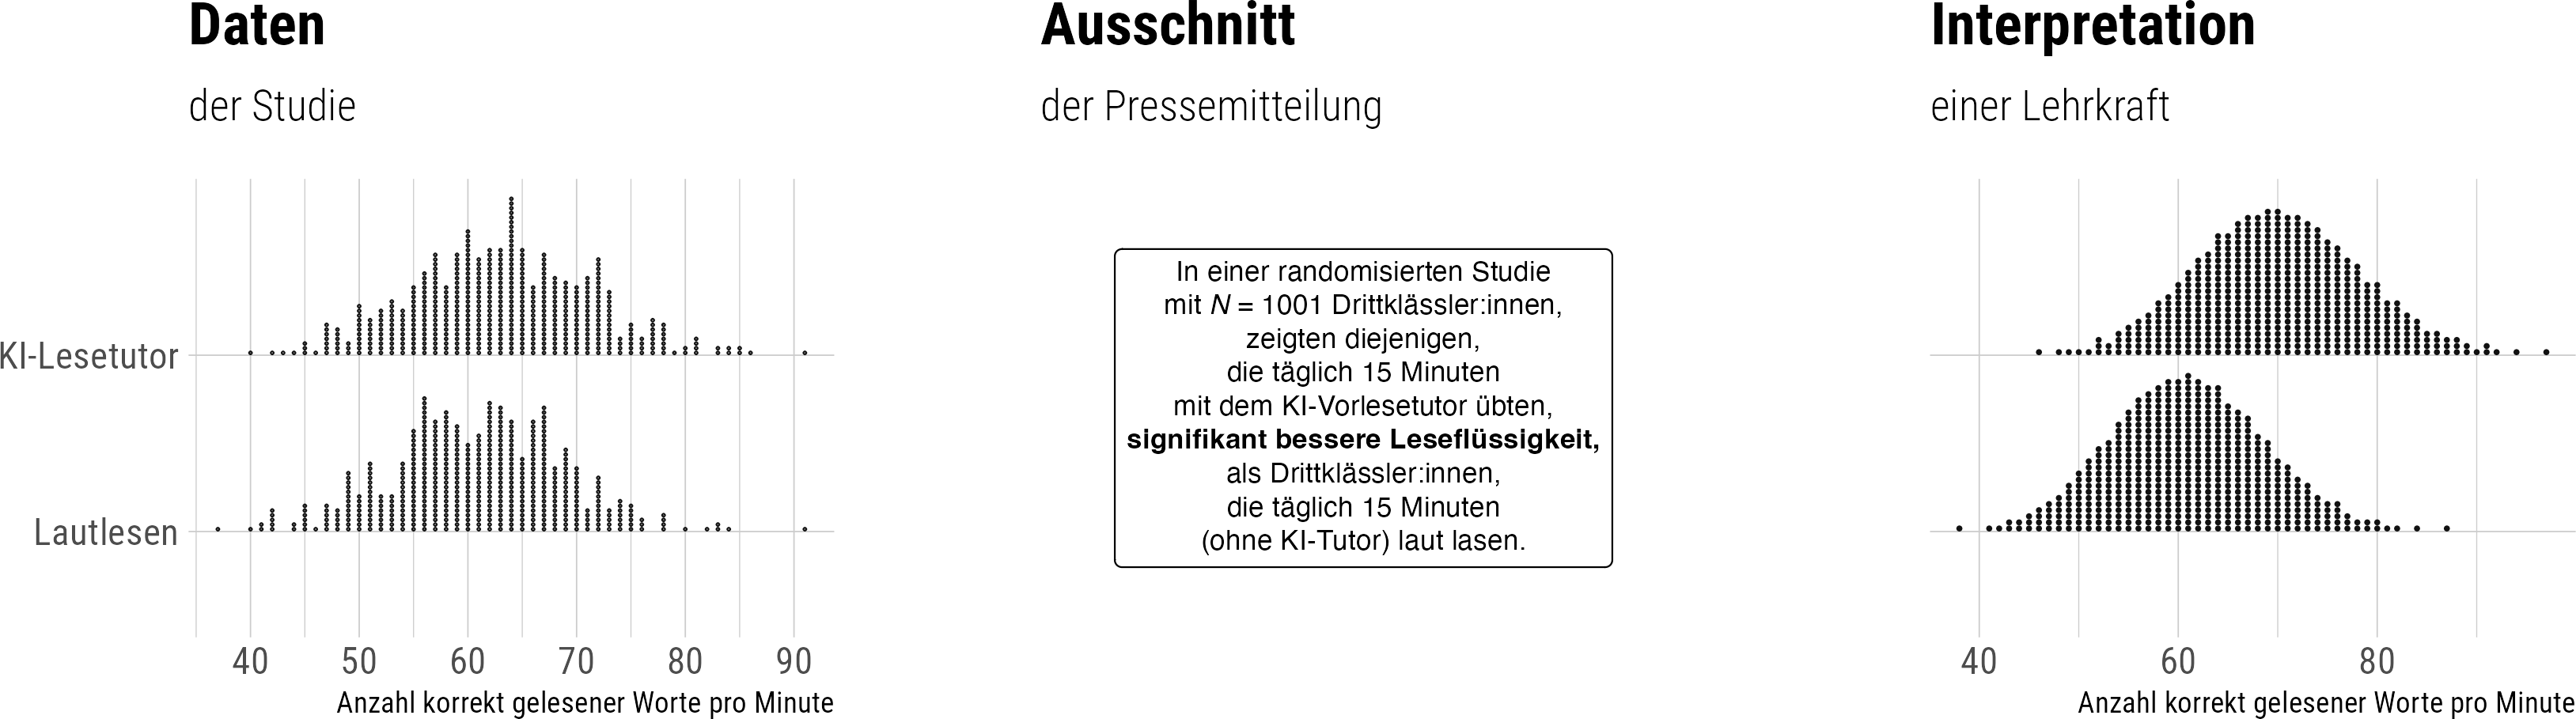
\includegraphics[keepaspectratio]{index_files/figure-pdf/fig-AbbildungMoMa-1.png}}

\end{figure*}

Liest eine Lehrkraft etwa die (fiktive) Pressemitteilung in
Abbildung~\ref{fig-AbbildungMoMa}, stellt sich die Ergebnisse wie in
Abbildung~\ref{fig-AbbildungMoMa} rechts vor
(\citeproc{ref-schmidt2023}{Schmidt et al., 2023}) und überzeugt
anschließend ihre Schulleitung diesen KI-Lesetutor zu beschaffen und
schulweit einzusetzen liegt höchstwahrscheinlich dysfunktionales
evidenzinformiertes Handeln vor. Denn die Forscher:innen bringen mit
\emph{signifikant bessere Leseflüssigkeit} zum Ausdruck, dass ihre Daten
unter der Annahme eines Nulleffekts unwahrscheinlich sind (signifikanter
p-Wert). Die Lehrkraft, jedoch interpretiert diese Formulierung als
»Unterschied bedeutsamer Größe«. Folglich schlussfolgert sie, dass es
Sinn macht geld und Zeit in Anschaffung und Implementation des
KI-Lesetutors zu investieren obwohl etwa die Implementation von
Lesetandems (\citeproc{ref-ehlert2024}{Ehlert et al., 2024})
kostengünstiger, weniger zeitaufwändig und lernwirksamer gewesen wäre.

Die Forschung zur Wissenschaftskommunikation hat eine Reihe solcher
potentiellen Problematiken aufgezeigt: Z.B. das soeben beschriebene
Verwechseln von Inferenzstatistik und Effektstärke
(\citeproc{ref-schmidt2023}{Schmidt et al., 2023}), das automatische
Annehmen starker Effekte, wenn keine Effektstärken berichtet wurden
(Practical Significance Bias, \citeproc{ref-michal2024}{Michal \& Shah,
2024}), Rückschaufehler (\citeproc{ref-masnick2009}{Masnick \&
Zimmerman, 2009}) oder die verzerrte Einschätzung der Belastbarkeit von
Befunden (z.B. Ergebnis einer Laborstudie mit \emph{N} = 56 mit großem
Effekt und daher hoher statistischer Power) durch irrelevante Zahlen
(z.B. Stichprobengröße einer zuvor gelesenen Large-Scale-Studie,
\citeproc{ref-bohrer2025}{Bohrer et al., 2025}).

Gleichzeitig liegt eine Reihe von Befunden vor, die implizieren, dass
verbesserte Kommunikation von Evidenz an Lehrkräfte zu Zwecken
evidenzinformierten Handelns vergleichsweise einfach umsetzbar ist.
Diese lassen sich zunächst in angebotsseitige und nutzendenseitige
Ansätze unterscheiden, also in Interventionen die die Auswahl und
Darstellung der Evidenz optimieren möchten und Ansätze die bei der
Scientific und Statistical Literacy der Lehrkräfte ansetzen.

\begin{tcolorbox}[enhanced jigsaw, leftrule=.75mm, opacityback=0, arc=.35mm, bottomtitle=1mm, coltitle=black, colframe=quarto-callout-caution-color-frame, toprule=.15mm, opacitybacktitle=0.6, colbacktitle=quarto-callout-caution-color!10!white, colback=white, toptitle=1mm, titlerule=0mm, left=2mm, rightrule=.15mm, breakable, bottomrule=.15mm, title=\textcolor{quarto-callout-caution-color}{\faFire}\hspace{0.5em}{Vorsicht}]

Gibt es diese Unterscheidung auch in der Literatur oder nur in unseren
Gesprächen?

\end{tcolorbox}

Zu zweiterem gehören Programme wie »Data Teams«
(\citeproc{ref-schildkamp2015}{Schildkamp \& Poortman, 2015}), welche
durch ein umfängliches Set an vordefinierten Leitlinien und Aktivitäten
versucht, konkrete schulische Probleme mit Hilfe von (oft eigens dafür
genierten) Daten zu lösen, wobei meist 4-6 Lehrkräfte und
Schulleiter:innen mit Bildungswissenschaftler:innen und
Fachdidaktiker:innen kooperieren. Auch kurz-
(\citeproc{ref-merk2020}{Merk et al., 2020}) oder längerfristig
angelegte (\citeproc{ref-karst2024}{Karst et al., 2024}) Interventionen
zur Anbahnung notwendiger Kompetenzen für evidenzinformiertes Handeln
wie Graph Literacy (\citeproc{ref-friel2001}{Friel et al., 2001}) oder
Forschungskompetenz (\citeproc{ref-neuenschwander2005}{Neuenschwander,
2005}) sowie die konkrete Unterstützung für solches
(\citeproc{ref-zotero-8935}{Academy, 2025}), können diesem Ansatz
zugerechnet werden.

Angebotsseitige Versuche die Kommunikation von Evidenz zu verbessern,
stammen aus verschiedensten sozialwissenschaftlichen Disziplinen: So
wird z.B. in der Psychologie untersucht, welche algebraisch äquivalenten
Formulierungen zu standardisierten Effektstärken bei Rezeption durch
Laien adäquatere Vorstellungen induzieren siehe~\ref{tbl-wisskommbsp}.
In der Human Computer Interaction Forschung werden (teils dynamische)
Visualisierungstechniken entwickelt, um Effektstärken und Inferential
Incertainty besser zu kommunizieren Zhang et al.
(\citeproc{ref-zhang2023}{2023}) und die bildungswissenschaftliche
Lehrerbildungsforschung sowie die Fachdidaktiken erproben innovative
Formate für die Zielgruppe der Lehrkräfte (z.B.
\citeproc{ref-schneider2024}{Schneider et al., 2024}), was auch das
anliegen der vorliegenden Studie ist.

\begin{ThreePartTable}

\begin{table}

\caption{\label{tbl-wisskommbsp}Beispiele für angebotsseitige Versuche
verbesserter Kommunikation von Evidenz}

\centering{

\fontsize{9.0pt}{10.8pt}\selectfont
\begin{tabular*}{\linewidth}{@{\extracolsep{\fill}}lll}
\toprule
 & Unterschied & Zusammenhang \\ 
\midrule\addlinespace[2.5pt]
Standard-kommunikation & Die Leseleistung von Schülerinnen und Schülern in  (PISA2022) sank um 28 Punkte und damit auf den Tiefststand. & Der sozioökonomische Status klärt 14\% der Varianz der Mathematikleistung auf. \\ 
Verbesserte Kommunikation & Die Leseleistungen von Schülerinnen und Schülern in Deutschland aus PISA2018 und aus PISA2022 überlappen sich zu 88,9\% wobei der Mittelwert um 28 Punkte sank. & Von 100 Schülerinnen und Schülern, die einen überdurchschnittlichen sozioökonomischen Status haben, zeigen 69 eine überdurchschnittliche Mathematikleistung. \\ 
\bottomrule
\end{tabular*}

}

\end{table}%

\end{ThreePartTable}

\section{Die vorliegende Studie}\label{die-vorliegende-studie}

In diesem Kontext untersucht die vorliegende Studie, inwiefern
verbreitete Standardgrafiken zur Kommunikation der Entwicklung der
Lesekompetenz in den deutschen Kohorten des Programme of International
Student Assessment (PISA) Practical Significance Bias induzieren und ob
dieser mit Grafiken eingedämmt werden kann, bei deren Gestaltung
theoretische und empirische Erkenntnisse der Wissenschaftkommunikation
siehe Abschnitt~\ref{sec-materialien} berücksichtigt wurden.

\subsection{Methode}\label{methode}

\subsubsection{Materialien}\label{sec-materialien}

In der Berichterstattung zu den Ergebnissen der PISA2022-Kohorte wurden
durch journalistische Medien zahlreiche Darstellungsformate gewählt,
insbesondere Line Graphs siehe Tabelle~\ref{tbl-pisalinegraphs}, was
angesichts der Anlage des PISA als Trendstudie
(\citeproc{ref-duxf6ring2016}{Döring \& Bortz, 2016}) konsequent
erscheint.

\begin{ThreePartTable}

\begin{longtable}[]{@{}
  >{\raggedright\arraybackslash}p{(\linewidth - 4\tabcolsep) * \real{0.3333}}
  >{\raggedright\arraybackslash}p{(\linewidth - 4\tabcolsep) * \real{0.3333}}
  >{\raggedright\arraybackslash}p{(\linewidth - 4\tabcolsep) * \real{0.3333}}@{}}
\caption{Verwendete Line Graphs in der
Berichterstattung.}\label{tbl-pisalinegraphs}\tabularnewline
\toprule\noalign{}
\endfirsthead
\endhead
\bottomrule\noalign{}
\endlastfoot
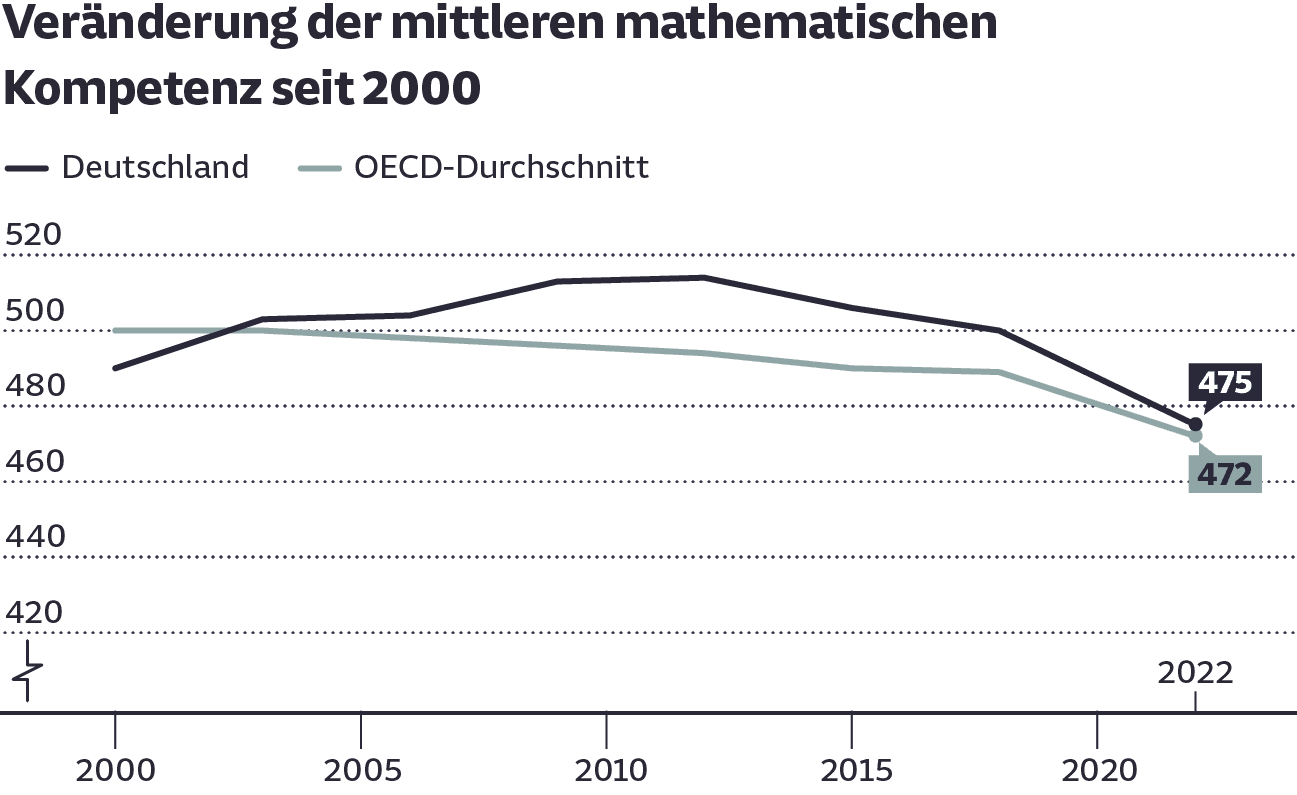
\includegraphics[width=9.375in,height=\textheight,keepaspectratio]{img/sz.png}
&
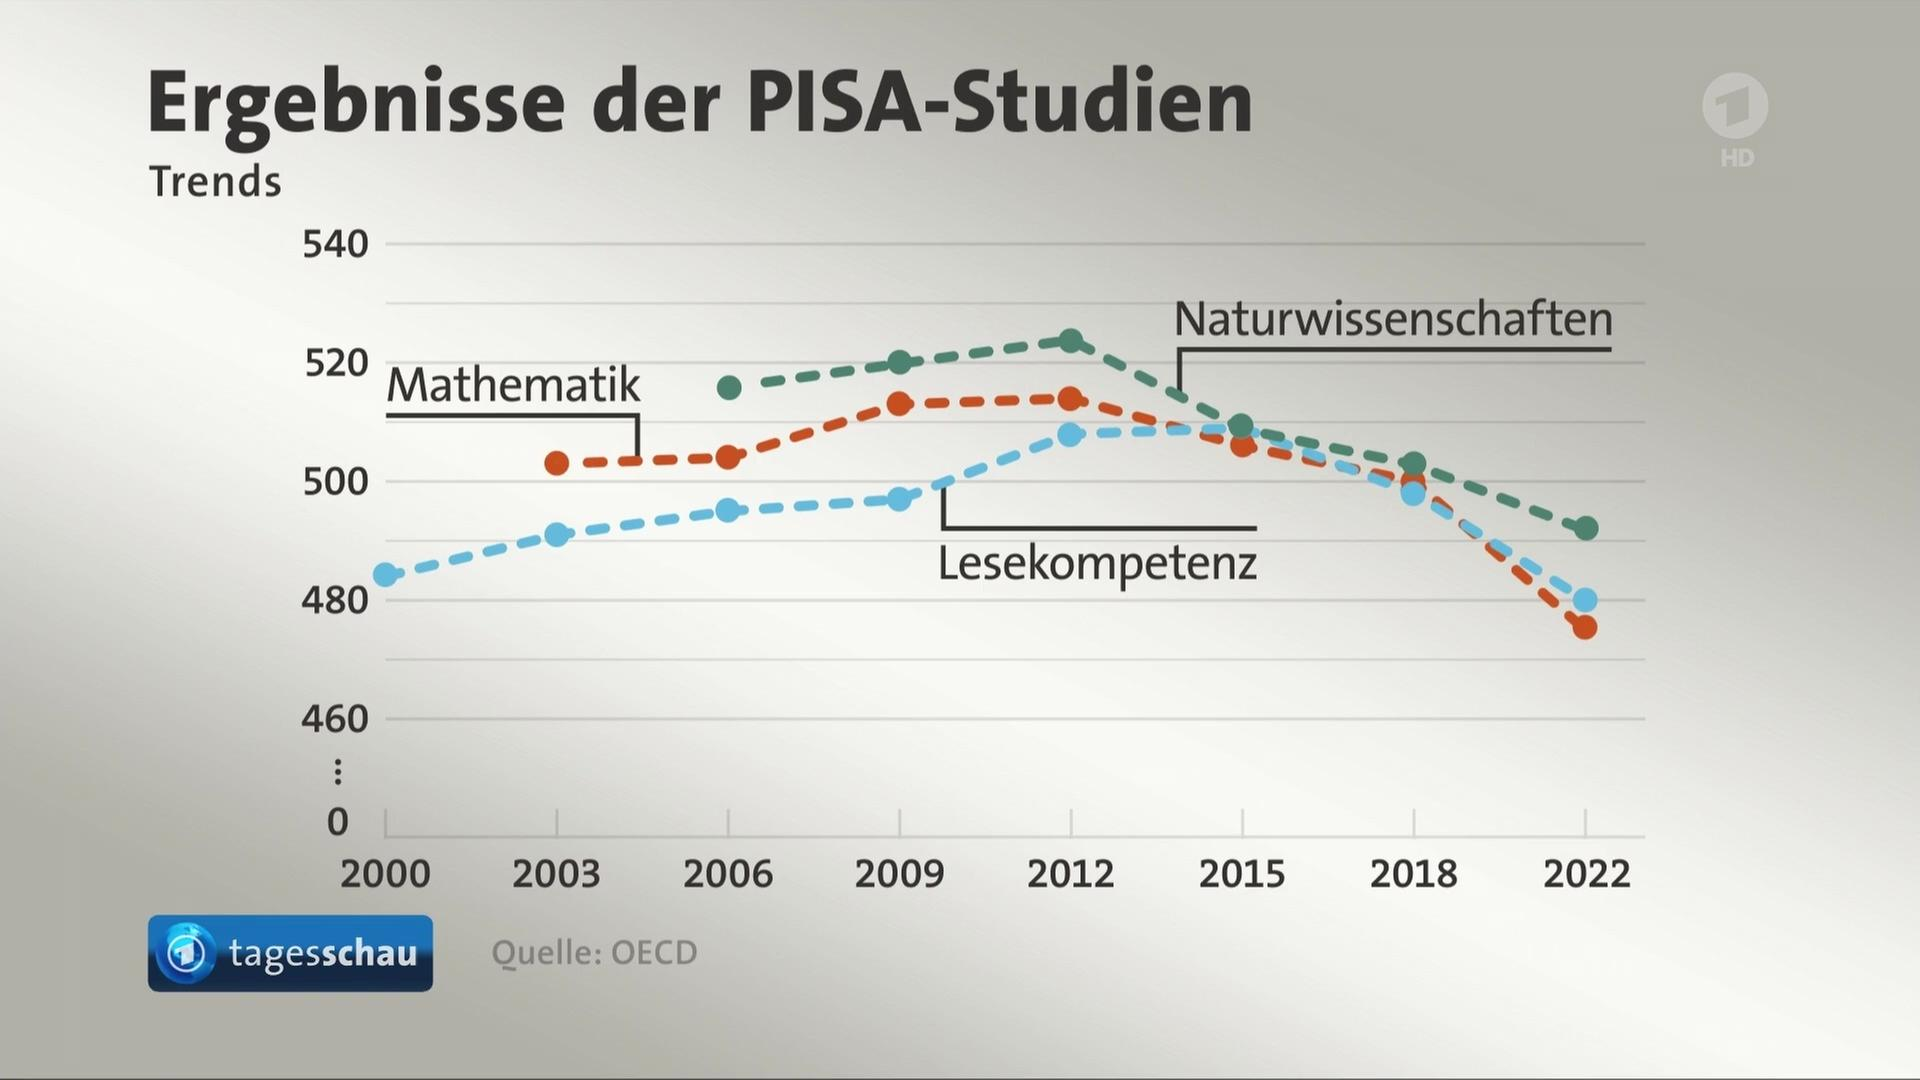
\includegraphics[width=9.375in,height=\textheight,keepaspectratio]{img/tagessschau.jpg}
&
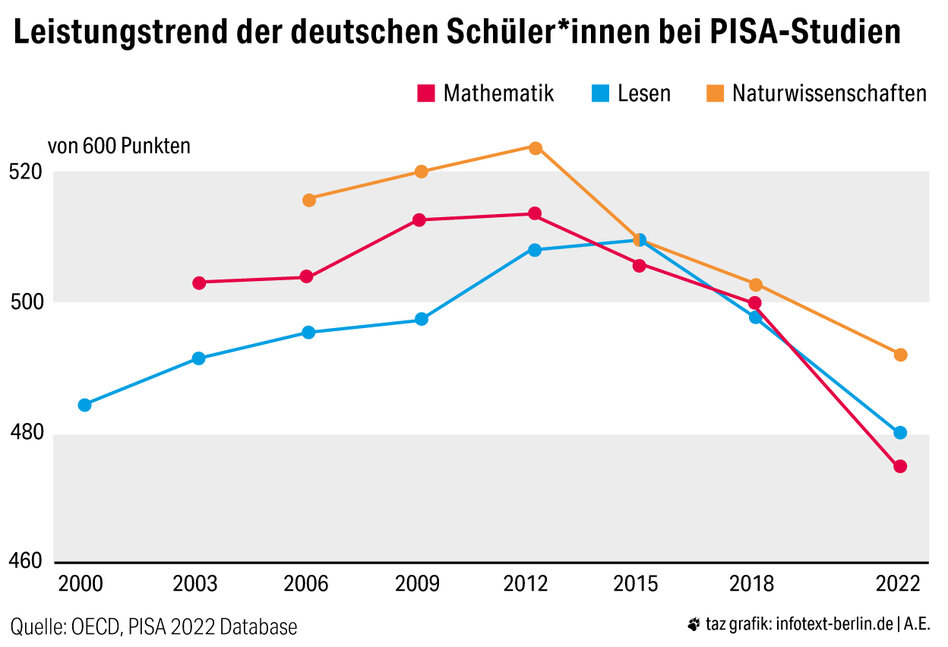
\includegraphics[width=8.33333in,height=\textheight,keepaspectratio]{img/taz.jpeg} \\
Süddeutsche Zeitung (\citeproc{ref-volkert2023}{2023}) & RBB
(\citeproc{ref-rbb2023}{2023}) & taz
(\citeproc{ref-taz.de2023}{2023}) \\
\end{longtable}

\end{ThreePartTable}

Diese Abbildungen erlauben einen effizienten Vergleich der Mittelwerte
sowohl über die Zeit als auch Variablen (hier: Fächer) hinweg. In
solchen Grafiken ist jedoch die Mittelwertsdifferenz nur bei bekannter
Streuung interpretierbar: Abbildung~\ref{fig-mwdiffstreuung} zeigt
jeweils die gleichen Mittelwertsdifferenzen von 508 (PISA Lesen 2015)
und 480 (PISA Lesen 2022).

\phantomsection\label{cell-fig-mwdiffstreuung}
\begin{figure*}[H]

{\caption{{Illustration der Unabhängigkeit von Mittelwertsdifferenz und
Größe des Effekts}{\label{fig-mwdiffstreuung}}}}

\pandocbounded{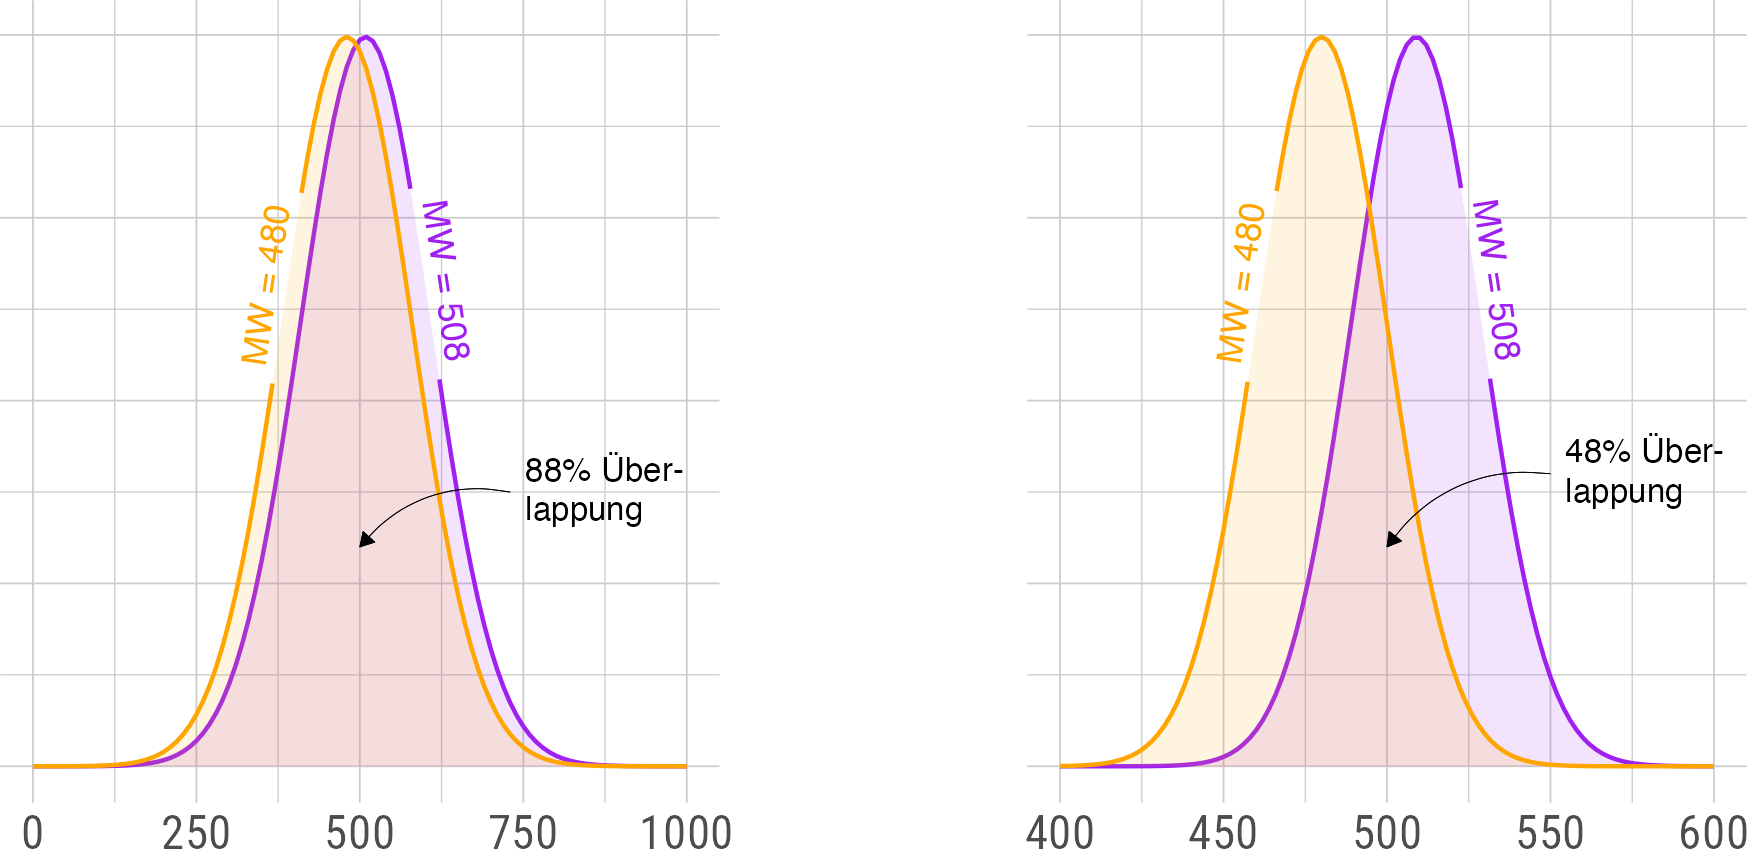
\includegraphics[keepaspectratio]{index_files/figure-pdf/fig-mwdiffstreuung-1.png}}

\end{figure*}

Das Ausmaß der Bedeutsamkeit dieses (gleichen) Mittelwertsunterschiedes
entsteht aber erst durch die Streuung der Daten um diesen Mittelwert
herum. Dadurch dass die Variablen im linken Teil der Abbildung kaum
streuen, ist die Überlappung der beiden Gruppen gering (48\%, großer
Effekt), während die große Überlappung im rechten Teil (88\%, kleiner
Effekt) durch die große Streuung zustande kommt. Die Abbildungen in
Tabelle~\ref{tbl-pisalinegraphs} sagen also nicht nur nichts über die
Bedeutsamkeit der Mittelwertsunterschiede aus - die nicht dargestellte
Varianz induziert womöglicherweise auch eine wahrgenommene große
Bedeutsamkeit der Mittelwertsdifferenz (\citeproc{ref-kale2020}{Kale et
al., 2020}).

\begin{ThreePartTable}

\begin{longtable}[]{@{}
  >{\raggedright\arraybackslash}p{(\linewidth - 2\tabcolsep) * \real{0.4444}}
  >{\raggedright\arraybackslash}p{(\linewidth - 2\tabcolsep) * \real{0.5556}}@{}}
\caption{Verwendete Stimuli}\label{tbl-materials}\tabularnewline
\toprule\noalign{}
\endfirsthead
\endhead
\bottomrule\noalign{}
\endlastfoot
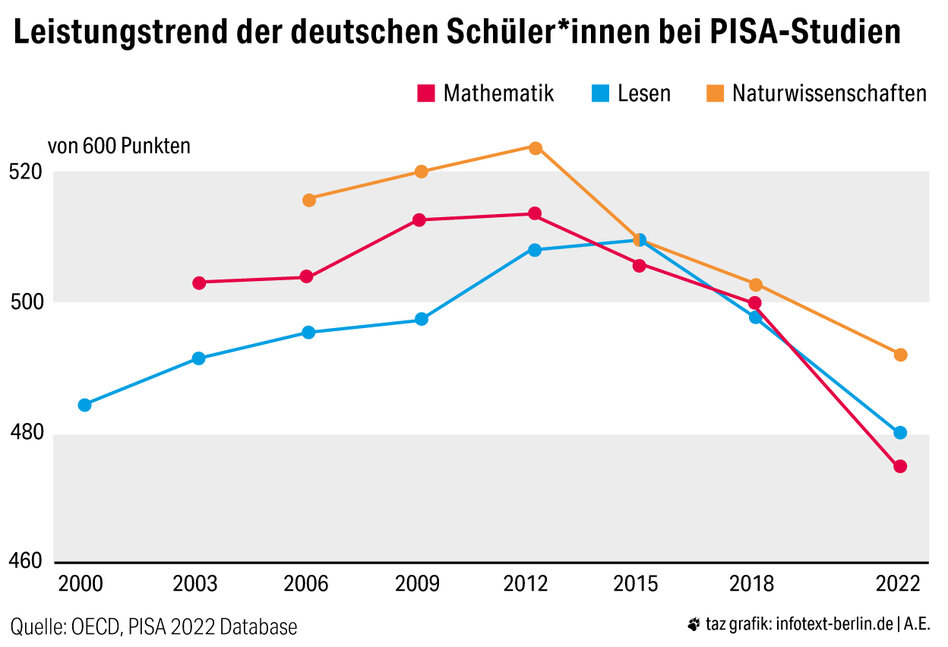
\includegraphics[width=4.16667in,height=\textheight,keepaspectratio]{img/taz.jpeg}
&
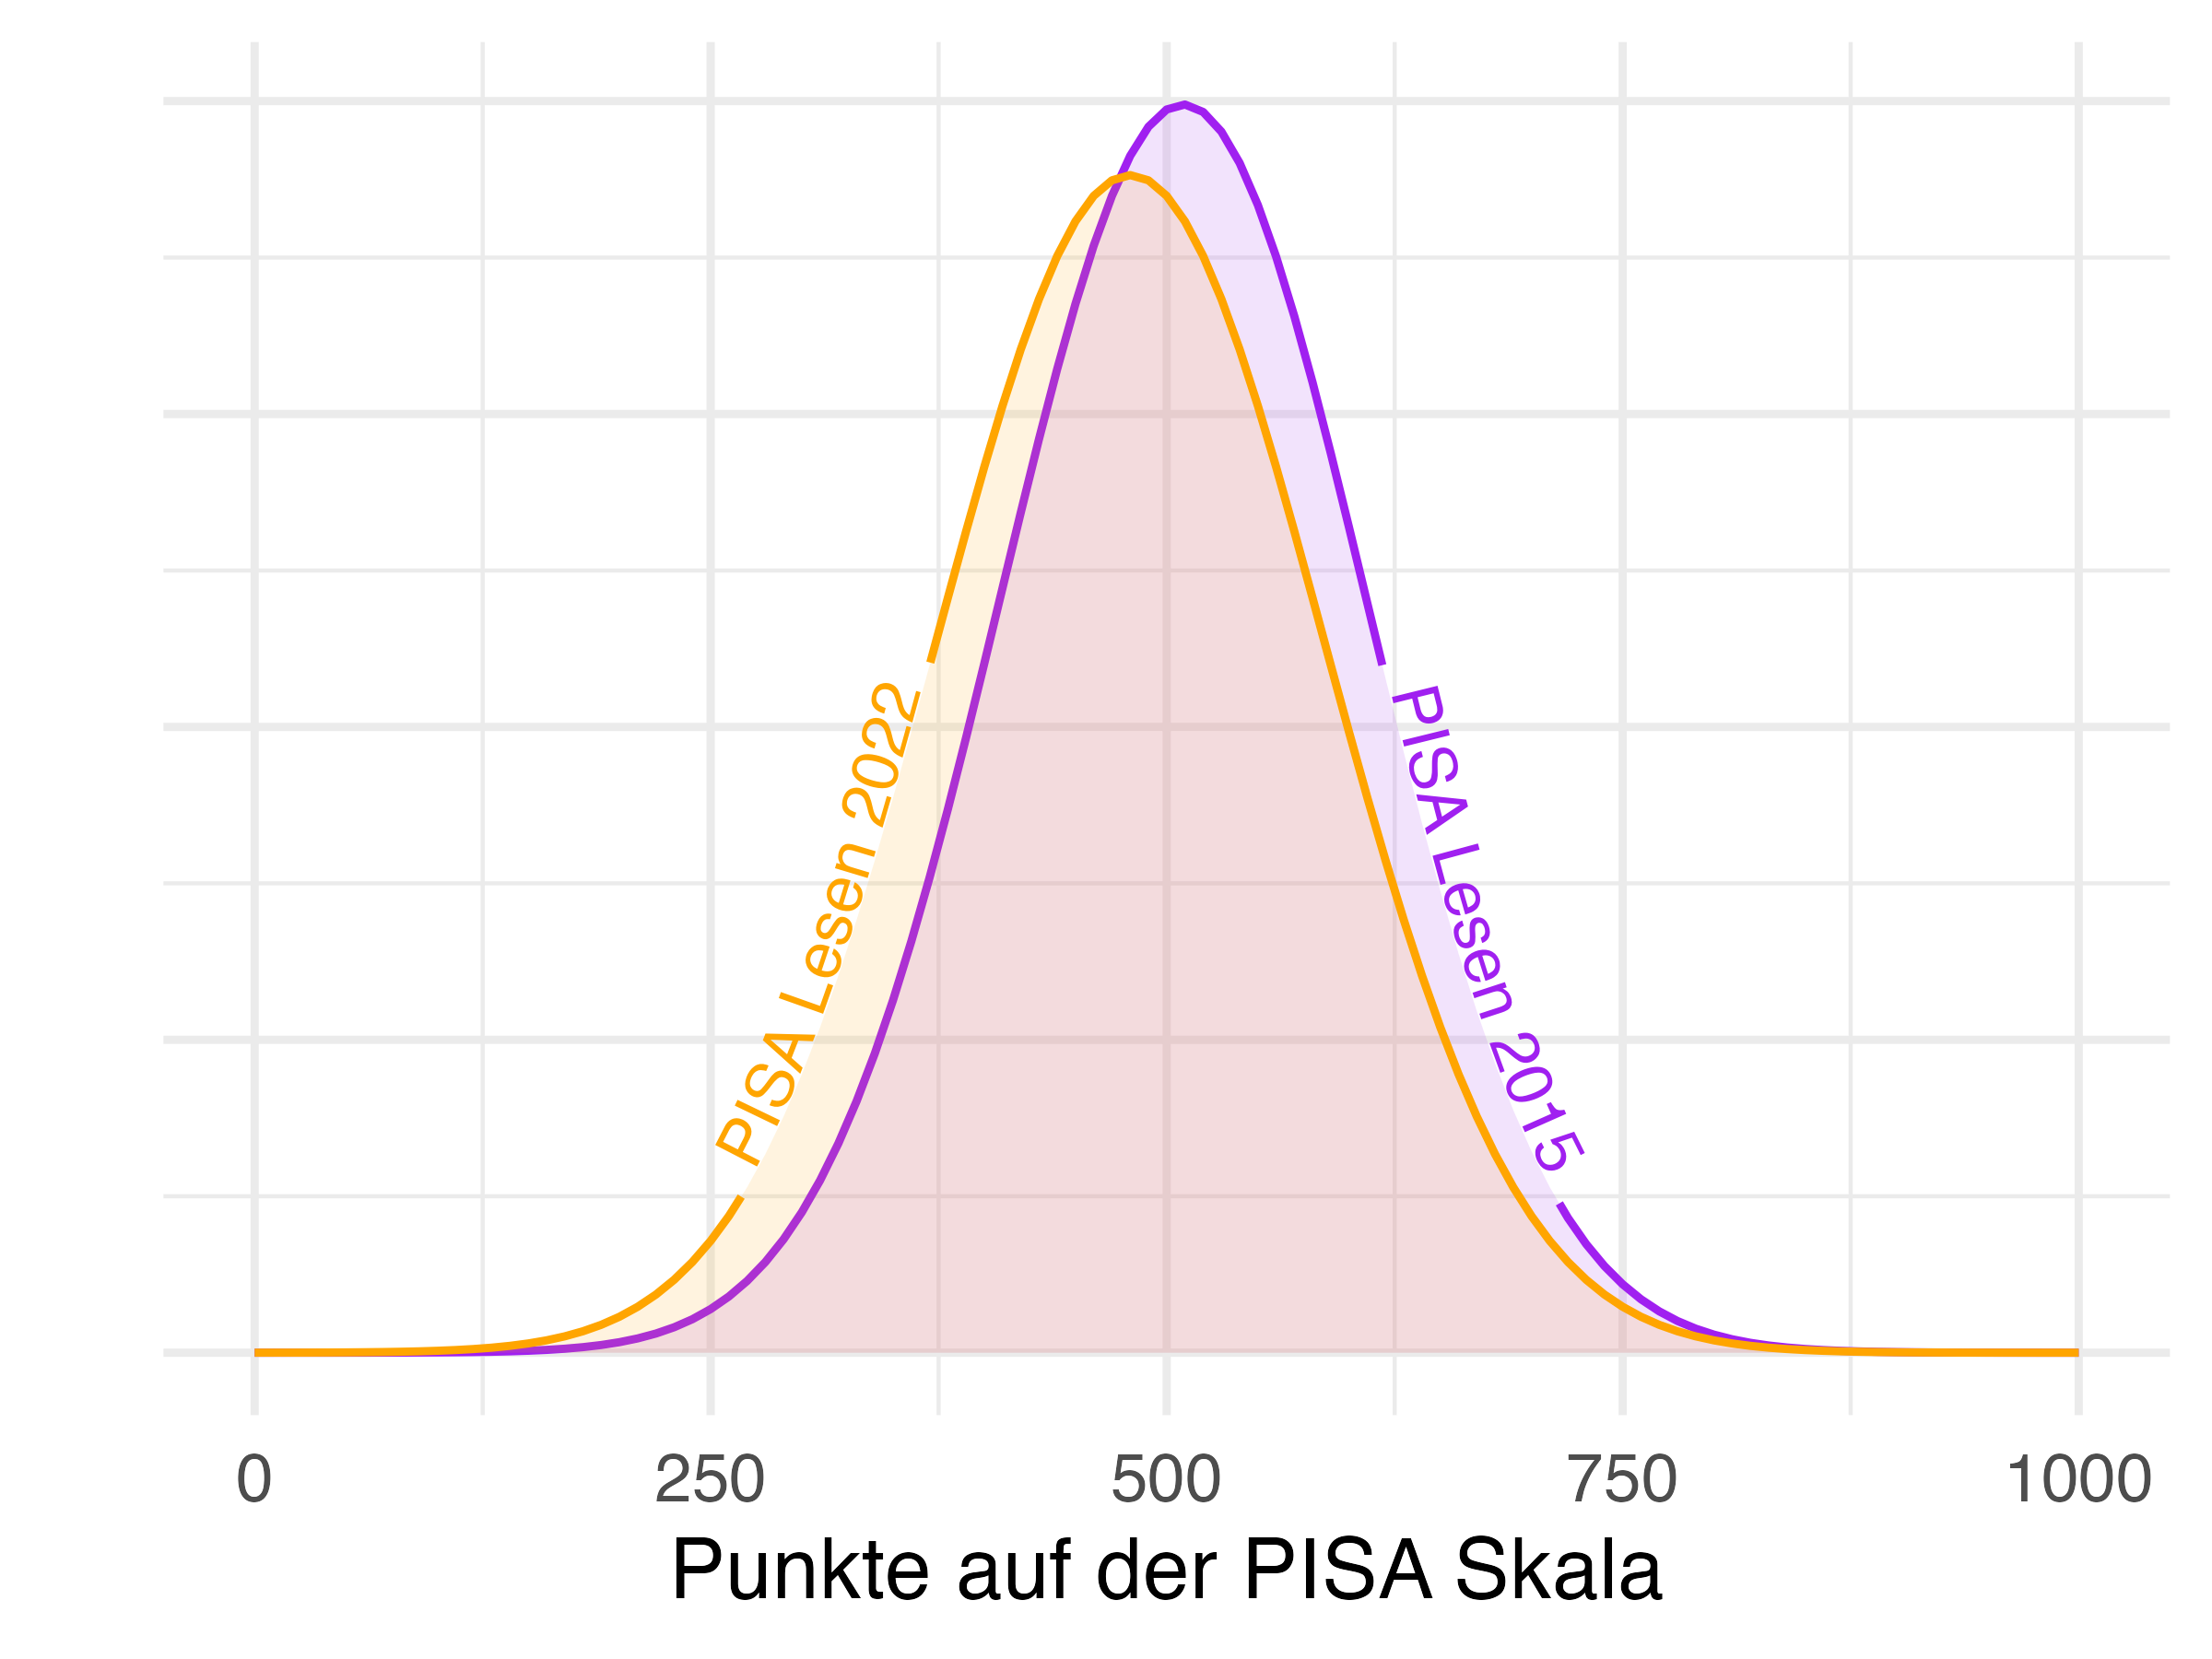
\includegraphics[width=3.78125in,height=\textheight,keepaspectratio]{img/geomtextline.png} \\
\end{longtable}

\end{ThreePartTable}

Daher wurden vorliegend neben Line Graphs auch überlappende
Verteilungskurven verwendet. Um diese barriereärmer zu gestalten wurde
bei der Farbgebung auf hinreichenden Kontrast bei den prävalenten
Sehbehinderungen geachtet (\citeproc{ref-garnier2023}{Garnier et al.,
2023}). Um unnötige Arbeitsgedächtnisbelastung zu vermeiden wurde die
Legende direkt in die Grafik integriert
(\citeproc{ref-franconeri2021}{Franconeri et al., 2021}).

\subsubsection{Design, Stichprobe und
Instrument}\label{design-stichprobe-und-instrument}

In einem einfachen between-person Design wurde \emph{N} = 216
Studierenden in Bachelorstudiengängen des Primar- und
Sekundarstufenlehramtes randomisiert eine der beiden in
Tabelle~\ref{tbl-materials} dargestellten Abbildungen gezeigt, um sie
mit folgenden Stimulus aufzufordern die Effektstärke einzuschätzen
``\emph{Basierend auf dieser Grafik: Wie hoch schätzen (exakte Antwort
nicht möglich) Sie die Wahrscheinlichkeit ein, dass eine zufällig
gezogene Schülerin oder ein zufällig gezogener Schüler aus dem Jahr 2022
im Lesen schlechter abschneidet als eine zufällig gezogene Schülerin
oder Schüler aus dem Jahr 2015}''. Beantwortet wurde diese Frage mit
einem Schieberegler, dessen Enden wie folgt beschriftet waren:
``\emph{50\% (beide Gruppen gleich)}'' und ``\emph{100\%}
\emph{(maximaler Effekt)}''. Diese Erfassung der wahrgenommenen
Effektstärke als »Probability of Superiority« ist der Human Computer
Interaction Forschung verbreitet und gilt als valide
(\citeproc{ref-brooks2014}{Brooks et al., 2014};
\citeproc{ref-kim2022}{Kim et al., 2022}), wenngleich die
Operationalisierung als Schieberegeler unklar lässt, inwiefern bei der
Beantwortung tatsächlich eine Elaboration der Überlappung vorgenommen
wird oder die Beantwortenden eher wie bei einem Likert-Item vorgehen.

\subsubsection{Statistische Analyse}\label{statistische-analyse}

Die abhängige Variable »Wahrgenommene Effektstärke« (operationalisiert
als Probability of Superiority) ist per Design auf das geschlossene
Intervall {[}0,5; 1{]} beschränkt und zeigt empirisch Bimodalität (siehe
Abbildung~\ref{fig-plotresults}). Um diesen Umständen in der
inferenzstatistischen Modellierung Rechnung zu tragen, wurden
bayesianische mixture Regressionsmodelle für zwei trunkierte
Normalverteilungen (\citeproc{ref-frischkorn2023}{Frischkorn \& Popov,
o.~J.}) in der probabilistischen Sprache Stan
(\citeproc{ref-standevelopmentteam2024}{Stan Development Team, 2024})
mithilfe des R-Pakets \{brms\} (\citeproc{ref-buxfcrkner2017}{Bürkner,
2017}) geschätzt.

\subsubsection{Ergebnisse}\label{ergebnisse}

Die Inspektion des Marcov-Chain-Monte-Carlo-Sampling-Prozesses zeigte
eine zufriedenstellende Qualität bzgl. der Konvergenz
\((\hat{R} < 1.01)\) und effektiver Sampling Size
(\(ESS_{Bulk} > 1000 < ESS_{Tail}\),
\citeproc{ref-vehtari2021prefix}{Vehtari et al., 2021}).

\phantomsection\label{cell-fig-plotresults}
\begin{figure*}[H]

{\caption{{Geschätze Effektstärke (Probability of Superiority) nach
Stimulus. Beide Gruppen zeigen einen sehr deutlichen Practicical
Significance Bias (Abstand von Median und wahrem
Wert).}{\label{fig-plotresults}}}}

\pandocbounded{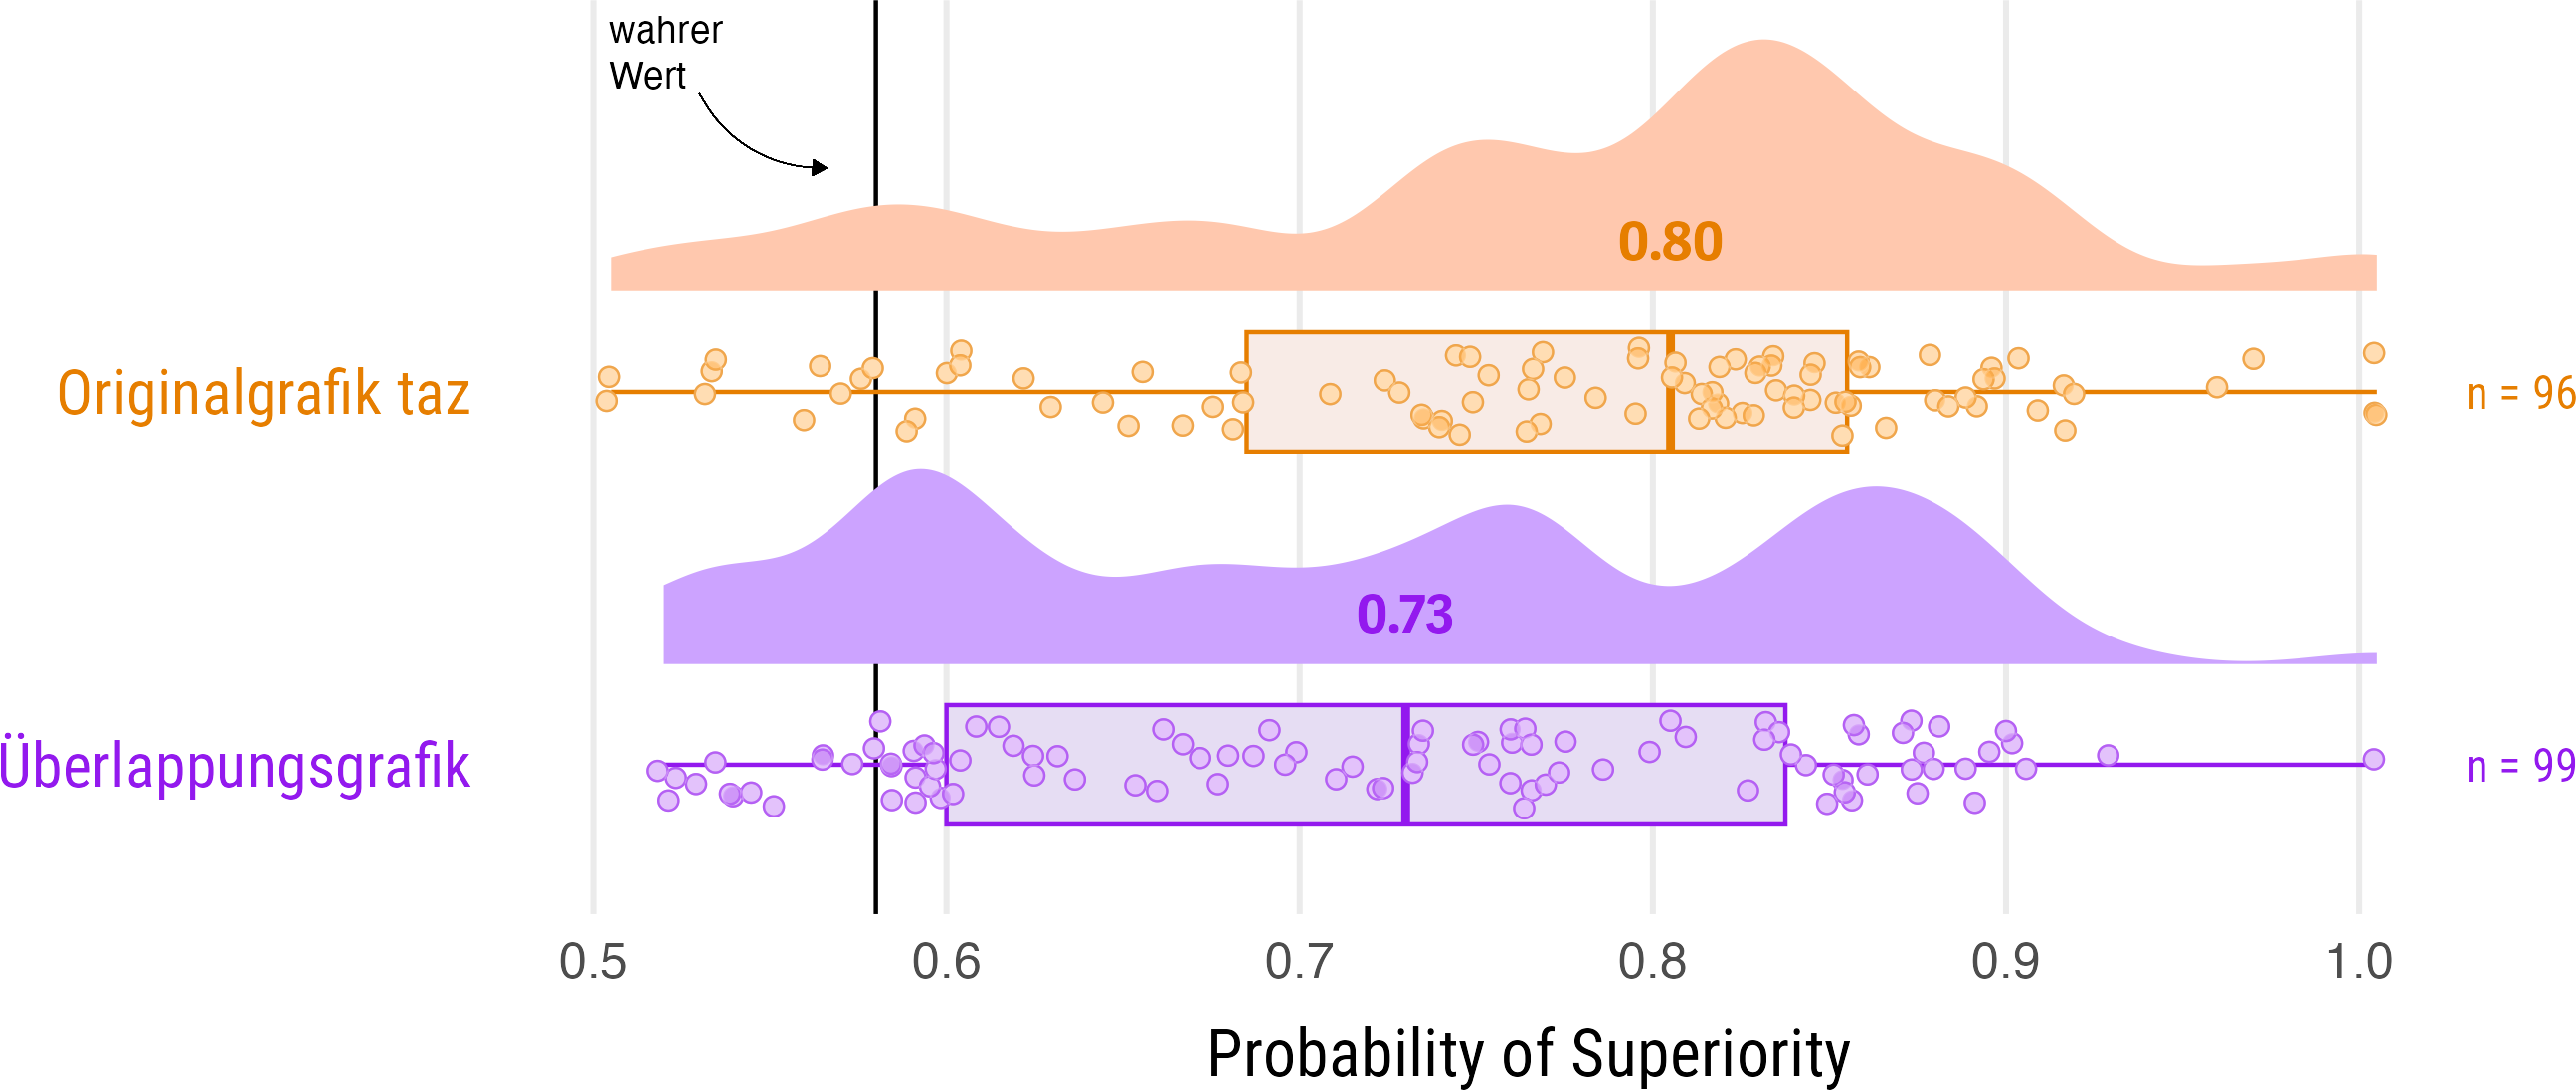
\includegraphics[keepaspectratio]{index_files/figure-pdf/fig-plotresults-1.png}}

\end{figure*}

Die Medianeinschätzung der Probability of Superiority betrug .80
(Originalgrafik) bzw. .73 (Überlappungsgrafik). Dieser Unterschied in
der Einschätzung entspricht einer Überlappung von 81.71\% (Cliff's
\emph{d} = 0) oder anders ausgedrückt: Legt man 100 mal einem:einer
Studierenden die Originalgrafik und einem:einer Studierenden die
Überlappungsgrafik vor, schätzt 61mal die:der Studierende mit der
Überlappungsgrafik den Effekt weniger verzerrt ein. Die
Inferenzstatistik für diesen Unterschied ist mit einer Evidence Ratio
von 14.8 klar konklusiv: Die vorliegenden Daten sind 14,8-fach
wahrscheinlicher unter der Annahme, dass der Mittelwert in der
geschätzten Effektstärke in der Gruppe mit der Überlappungsgrafik
niedriger ist als unter der Annahme, dass beide gleich sind.

\section{Diskussion}\label{diskussion}

\subsection{Literatur}\label{literatur}

\phantomsection\label{refs}
\begin{CSLReferences}{1}{0}
\bibitem[\citeproctext]{ref-zotero-8935}
Academy, C. H. U. (2025). \emph{Clearing House Unterricht Academy}.
\url{https://clearinghouse-academy.de/}

\bibitem[\citeproctext]{ref-aero2023}
AERO. (2023). \emph{Evidence-based teaching practices}.

\bibitem[\citeproctext]{ref-altrichter2006}
Altrichter, H., \& Rolff, H.-G. (2006). Datenbasierte Schulentwicklung.
Editorial. \emph{Journal für Schulentwicklung}, \emph{10}(4), 4--6.

\bibitem[\citeproctext]{ref-bauer2012}
Bauer, J., \& Prenzel, M. (2012). European teacher training reforms.
\emph{Science}, \emph{336}(6089), 1642--1643.
\url{https://doi.org/10.1126/science.1218387}

\bibitem[\citeproctext]{ref-bauer1978}
Bauer, K.-O., \& Rolff, H.-G. (1978). \emph{Vorarbeiten zu einer Theorie
der Schulentwicklung} (K.-O. Bauer \& H.-G. Rolff, Hrsg.; S. 219--263).
Beltz.

\bibitem[\citeproctext]{ref-bellmann2011}
Bellmann, J., \& Müller, T. (2011). \emph{Evidenzbasierte Pädagogik
{\textendash} ein Déjà-vu?} (J. Bellmann \& T. Müller, Hrsg.; S. 9--32).
VS Verlag für Sozialwissenschaften.
\url{https://doi.org/10.1007/978-3-531-93296-5_1}

\bibitem[\citeproctext]{ref-biesta2007}
Biesta, G. (2007). Why {``}What Works{''} Won{'}t Work: Evidence-Based
Practice and the Democratic Deficit in Educational Research.
\emph{Educational Theory}, \emph{57}(1), 1--22.
\url{https://doi.org/10.1111/j.1741-5446.2006.00241.x}

\bibitem[\citeproctext]{ref-bohl2020}
Bohl, T. (2020). \emph{Theorien der Schulentwicklung} (M. Harant, P.
Thomas, \& U. Küchler, Hrsg.; S. 97--109). Tübingen University Press.
\url{https://doi.org/10.15496/publikation-45627}

\bibitem[\citeproctext]{ref-bohrer2025}
Bohrer, K., Schmidt, K., \& Merk, S. (2025). Zwei Studien, ein Ergebnis:
Lehramtsstudierende unterliegen im Umgang mit Evidenz dem Ankereffekt.
\emph{Zeitschrift für Erziehungswissenschaft}.

\bibitem[\citeproctext]{ref-bromme2014b}
Bromme, R., Prenzel, M., \& Jäger, M. (2014). Empirische
{Bildungsforschung} Und Evidenzbasierte {Bildungspolitik}. In
\emph{Zeitschrift für Erziehungswissenschaft} (Bd. 17).
\url{https://doi.org/10.1007/s11618-014-0514-5}

\bibitem[\citeproctext]{ref-brooks2014}
Brooks, M. E., Dalal, D. K., \& Nolan, K. P. (2014). Are common language
effect sizes easier to understand than traditional effect sizes?
\emph{Journal of Applied Psychology}, \emph{99}(2), 332--340.
\url{https://doi.org/10.1037/a0034745}

\bibitem[\citeproctext]{ref-bruegelmann2018}
Brügelmann, H. (2018). \emph{Unterrichts- und Schulentwicklung in
Communities of Practice} (H. Barz, Hrsg.; S. 479--484). Springer
Fachmedien. \url{https://doi.org/10.1007/978-3-658-07491-3_44}

\bibitem[\citeproctext]{ref-buxfcrkner2017}
Bürkner, P.-C. (2017). brms: An R Package for Bayesian Multilevel Models
Using Stan. \emph{Journal of Statistical Software}, \emph{80}(1).
\url{https://doi.org/10.18637/jss.v080.i01}

\bibitem[\citeproctext]{ref-eurlex2024}
Council of the European Union. (2024). \emph{Council conclusions on
promoting evidence-informed policy and practice in education and
training to achieve the European Education Area}.
\url{https://eur-lex.europa.eu/legal-content/EN/TXT/PDF/?uri=OJ:C_202403642}

\bibitem[\citeproctext]{ref-duxf6ring2016}
Döring, N., \& Bortz, J. (2016). \emph{Forschungsmethoden und Evaluation
in den Sozial- und Humanwissenschaften} (5., vollst). Springer.
\url{http://dx.doi.org/10.1007/978-3-642-41089-5}

\bibitem[\citeproctext]{ref-ehlert2024}
Ehlert, M., Beck, J., Förster, N., \& Souvignier, E. (2024). Continuous
texts or word lists? Exploring the effects and the process of repeated
reading depending on the reading material and students{'} reading
abilities. \emph{Reading and Writing}.
\url{https://doi.org/10.1007/s11145-024-10536-5}

\bibitem[\citeproctext]{ref-franconeri2021}
Franconeri, S. L., Padilla, L. M., Shah, P., Zacks, J. M., \& Hullman,
J. (2021). The science of visual data communication: What works.
\emph{Psychological Science in the Public Interest}, \emph{22}(3),
110--161. \url{https://doi.org/10.1177/15291006211051956}

\bibitem[\citeproctext]{ref-friel2001}
Friel, S. N., Curcio, F. R., \& Bright, G. W. (2001). Making sense of
graphs: Critical factors influencing comprehension and instructional
implications. \emph{Journal for Research in Mathematics Education},
\emph{32}(2), 124. \url{https://doi.org/10.2307/749671}

\bibitem[\citeproctext]{ref-frischkorn2023}
Frischkorn, G. T., \& Popov, V. (o.~J.). \emph{A Tutorial for Estimating
Bayesian hierarchical mixture models for visual working memory tasks:
Introducing the Bayesian Measurement Modeling (bmm) package for R}.
\url{https://doi.org/10.31234/osf.io/umt57}

\bibitem[\citeproctext]{ref-garnier2023}
Garnier, S., Ross, N., BoB Rudis, Filipovic-Pierucci, A., Galili, T.,
Timelyportfolio, O'Callaghan, A., Greenwell, B., Sievert, C., Harris, D.
J., Sciaini, M., \& JJ Chen. (2023). \emph{sjmgarnier/viridis: CRAN
release v0.6.3}. Zenodo. \url{https://doi.org/10.5281/ZENODO.4679423}

\bibitem[\citeproctext]{ref-grouxdfophoff2023}
Groß Ophoff, J., Brown, C., \& Helm, C. (2023). Do pupils at
research-informed schools actually perform better? Findings from a study
at English schools. \emph{Frontiers in Education}, \emph{7}, 1011241.
\url{https://doi.org/10.3389/feduc.2022.1011241}

\bibitem[\citeproctext]{ref-hau2012}
Hau, R., Martini, U., \& Dralle, A. (2012). \emph{PONS Wörterbuch für
Schule und Studium Latein-Deutsch}. PONS.

\bibitem[\citeproctext]{ref-helmke2022}
Helmke, A. (2022). \emph{Unterrichtsqualität und Professionalisierung:
Diagnostik von Lehr-Lern-Prozessen und evidenzbasierte
Unterrichtsentwicklung}. Klett Kallmeyer.

\bibitem[\citeproctext]{ref-holtappels2007}
Holtappels, H. G. (2007). \emph{Schulentwicklungsprozesse und Change
Management. Innovationstheoretische Reflexionen und Forschungsbefunde
über Steuergruppen.} (N. Berkemeyer, Hrsg.; S. 11--39). Juventa.

\bibitem[\citeproctext]{ref-hullman2015}
Hullman, J., Resnick, P., \& Adar, E. (2015). Hypothetical outcome plots
outperform error bars and violin plots for inferences about reliability
of variable ordering. \emph{PLOS ONE}, \emph{10}(11), e0142444.
\url{https://doi.org/10.1371/journal.pone.0142444}

\bibitem[\citeproctext]{ref-jones2024}
Jones, A. (2024). Rethinking Evidence-Based Practice in Education: A
Critical Literature Review of the {`}What Works{'} Approach.
\emph{International Journal of Educational Researchers}, \emph{15}(2),
37--51. \url{https://doi.org/10.29329/ijer.2024.1041.3}

\bibitem[\citeproctext]{ref-kale2020}
Kale, A., Kay, M., \& Hullman, J. (2020). \emph{Visual reasoning
strategies for effect size judgments and decisions}.
\url{https://doi.org/10.48550/ARXIV.2007.14516}

\bibitem[\citeproctext]{ref-karst2024}
Karst, K., Yendell, O., Marx, A., Lettau, W.-D., \& Hawlitschek, P.
(2024). \emph{Die Etablierung von Evidenzteams in SchuMaS {\textendash}
Eine Strategie zur systematischen Nutzung von Daten für die Schul- und
Unterrichtsentwicklung} (K. Maaz \& A. Marx, Hrsg.; S. 225--240).
Waxmann. \url{https://madoc.bib.uni-mannheim.de/67727/}

\bibitem[\citeproctext]{ref-kelly2023}
Kelly, M. G., \& Farrie, D. (2023). Misrepresented Funding Gaps in Data
for Some States. \emph{Educational Researcher}, \emph{52}(4), 244--247.
\url{https://doi.org/10.3102/0013189X221133396}

\bibitem[\citeproctext]{ref-kim2022}
Kim, Y.-S., Hofman, J. M., \& Goldstein, D. G. (2022). \emph{CHI '22:
CHI Conference on Human Factors in Computing Systems}. 1--14.
\url{https://doi.org/10.1145/3491102.3502053}

\bibitem[\citeproctext]{ref-kluge2011}
Kluge, F. (2011). \emph{Etymologisches Wörterbuch der deutschen Sprache}
(25. Aufl.). De Gruyter.

\bibitem[\citeproctext]{ref-masnick2009}
Masnick, A. M., \& Zimmerman, C. (2009). Evaluating scientific research
in the context of prior belief: Hindsight bias or confirmation bias?
\emph{Journal of Psychology of Science and Technology}, \emph{2}(1),
29--36. \url{https://doi.org/10.1891/1939-7054.2.1.29}

\bibitem[\citeproctext]{ref-merk2020}
Merk, S., Poindl, S., Wurster, S., \& Bohl, T. (2020). Fostering Aspects
of Pre-Service Teachers' Data Literacy: {Results} of a Randomized
Controlled Trial. \emph{Teaching and Teacher Education}, \emph{91},
103043. \url{https://doi.org/10.1016/j.tate.2020.103043}

\bibitem[\citeproctext]{ref-michal2024}
Michal, A. L., \& Shah, P. (2024). A Practical Significance Bias in
Laypeople{'}s Evaluation of Scientific Findings. \emph{Psychological
Science}, 09567976241231506.
\url{https://doi.org/10.1177/09567976241231506}

\bibitem[\citeproctext]{ref-neuenschwander2005}
Neuenschwander, M. P. (2005). Forschungskompetenzen in der Lehrerinnen-
und Lehrerbildung erweitern: Ein Weiterbildungskonzept. \emph{BzL -
Beiträge zur Lehrerinnen- und Lehrerbildung}, \emph{23}(2), 270--280.
\url{https://doi.org/10.36950/bzl.23.2.2005.10132}

\bibitem[\citeproctext]{ref-pellegrini2021}
Pellegrini, M., \& Vivanet, G. (2021). Evidence-Based Policies in
Education: Initiatives and Challenges in Europe. \emph{ECNU Review of
Education}, \emph{4}(1), 2545.
\url{https://doi.org/10.1177/2096531120924670}

\bibitem[\citeproctext]{ref-rbb2023}
RBB, M. K. (2023). \emph{Deutsche Schülerinnen und Schüler schneiden bei
neuer PISA-Studie so schlecht ab wie nie zuvor}.
\url{https://www.tagesschau.de/multimedia/video/video-1280422.html}

\bibitem[\citeproctext]{ref-renkl2022}
Renkl, A. (2022). Meta-analyses as a privileged information source for
informing teachers' practice? A plea for theories as primus inter pares.
\emph{Zeitschrift Für Pädagogische Psychologie}, \emph{36}(4), 217--231.
\url{https://doi.org/10.1024/1010-0652/a000345}

\bibitem[\citeproctext]{ref-schildkamp2015}
Schildkamp, K., \& Poortman, C. L. (2015). Factors influencing the
functioning of data teams. \emph{Teachers College record},
\emph{117}(4), 1--42.
\url{https://doi.org/10.1080/09243453.2016.1256901}

\bibitem[\citeproctext]{ref-schmidt2024}
Schmidt, K. (2024). \emph{Teachers{'} Engagement With Educational
Science How to Communicate Findings From Educational Science in a
User-Friendly Way to Teachers} {[}Phdthesis{]}.

\bibitem[\citeproctext]{ref-schmidt2023}
Schmidt, K., Edelsbrunner, P. A., Rosman, T., Cramer, C., \& Merk, S.
(2023). When perceived informativity is not enough. How teachers
perceive and interpret statistical results of educational research.
\emph{Teaching and Teacher Education}, \emph{130}, 104134.
\url{https://doi.org/10.1016/j.tate.2023.104134}

\bibitem[\citeproctext]{ref-schneider2024}
Schneider, J., Schmidt, K., Bohrer, K., \& Merk, S. (2024).
Communicating Effect Sizes to Teachers. \emph{Zeitschrift Für
Psychologie}.
\url{https://econtent.hogrefe.com/doi/10.1027/2151-2604/a000573}

\bibitem[\citeproctext]{ref-shavelson2002}
Shavelson, R. J., \& Towne, L. (2002). \emph{Scientific Research in
Education}. National Academies Press.

\bibitem[\citeproctext]{ref-slavin2020}
Slavin, R. E. (2020). How evidence-based reform will transform research
and practice in education. \emph{Educational Psychologist},
\emph{55}(1), 21--31.
\url{https://doi.org/10.1080/00461520.2019.1611432}

\bibitem[\citeproctext]{ref-standevelopmentteam2024}
Stan Development Team. (2024). \emph{Stan Modeling Language Users Guide
and Reference Manual}. \url{https://mc-stan.org}

\bibitem[\citeproctext]{ref-stark2017}
Stark, R. (2017). Probleme evidenzbasierter bzw. -orientierter
pädagogischer Praxis. \emph{Zeitschrift für Pädagogische Psychologie},
\emph{31}(2), 99--110. \url{https://doi.org/10.1024/1010-0652/a000201}

\bibitem[\citeproctext]{ref-taz.de2023}
taz.de. (2023). \emph{Pisa-Schock für deutsche Schü­le­r:in­nen: Im freien
Fall \textbar{} taz.de}.
\url{https://taz.de/Pisa-Schock-fuer-deutsche-Schuelerinnen/!5974146/}

\bibitem[\citeproctext]{ref-thorndike1904}
Thorndike, E. L. (1904). \emph{Theory of mental and social
measurements.} The Science Press.
\url{https://doi.org/10.1037/13283-000}

\bibitem[\citeproctext]{ref-vehtari2021prefix}
Vehtari, A., Gelman, A., Simpson, D., Carpenter, B., \& Bürkner, P.-C.
(2021). Rank-Normalization, Folding, and Localization: An Improved Rˆ
for Assessing Convergence of MCMC (with Discussion). \emph{Bayesian
Analysis}, \emph{16}(2). \url{https://doi.org/10.1214/20-BA1221}

\bibitem[\citeproctext]{ref-volkert2023}
Volkert, L., \& Germany, S. de G., Munich. (2023). \emph{Jeder dritte
15-Jährige scheitert an leichten Mathe-Aufgaben}.
\url{https://www.sueddeutsche.de/projekte/artikel/politik/pisa-studie-schulen-mathe-aufgaben-jugendliche-scheitern-gruende-e206264/}

\bibitem[\citeproctext]{ref-zhang2023}
Zhang, S., Heck, P. R., Meyer, M. N., Chabris, C. F., Goldstein, D. G.,
\& Hofman, J. M. (2023). An illusion of predictability in scientific
results: Even experts confuse inferential uncertainty and outcome
variability. \emph{Proceedings of the National Academy of Sciences},
\emph{120}(33), e2302491120.
\url{https://doi.org/10.1073/pnas.2302491120}

\end{CSLReferences}






\end{document}
